\chapter{Design}\label{design}


%------------------------------------------------------
\section{Architecture}\label{architecture}


\section{Workflow}\label{workflow}

\subsection{Import}\label{workflow-import}

\begin{figure}[h]
  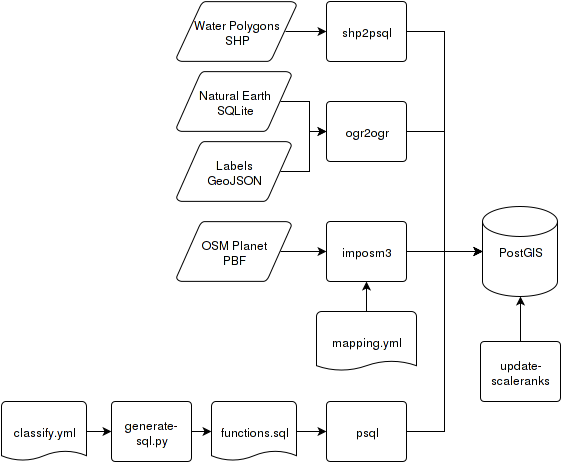
\includegraphics[scale=0.6]{images/import_flow.png}
  \caption{Import workflow from various data sources into PostGIS}
\end{figure}

\subsection{Export}\label{workflow-export}

\begin{figure}[h]
  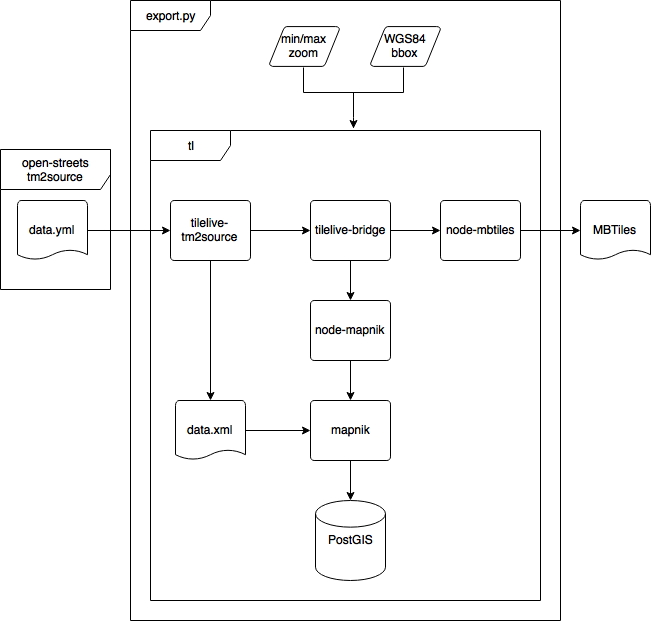
\includegraphics[scale=0.6]{images/export_flow.png}
  \caption{Export data from PostGIS to MBTiles}
\end{figure}

%------------------------------------------------------
\section{Database Schema}\label{database-schema}


The schema is flat and has no relations. Each table contains
information about its entity and geometry. Because imposm 3
cannot match two types of polygons (e.g. polygon and point) we need
to create a table for each geometry type.


\subsection{Common Attributes}

\subsubsection{OSM id}

All tables and views that are derived from \osm{} data have keep the original \texttt{osm\_id}
to trace back the data and be able to query a distinct \osm{} feature in a visual style.

\subsubsection{Translations}

All features that will get a label layer will contain several translations.

\begin{flushleft}
\begin{table}
    \begin{tabular}{ll}
    \hline
     Field    & 	Description                                    \\
    \hline
    name      & Local name for the place.  \\
    name\_en	 & English                          \\
    name\_es	 & Spanish                          \\
    name\_fr	 & French                           \\
    name\_de	 & German                           \\
    name\_ru	 & Russian                          \\
    name\_zh	 & Chinese                          \\
    \end{tabular}
\end{table}
\end{flushleft}


\subsubsection{Type and Class}

The class can be explained as a feature class. It is a categorization of a OSM value.
The type is the OSM value of the feature.


\subsection{OpenStreetMap Planet}

\begin{flushleft}
    \begin{tabular}{lll}
    \hline
    Table Name            & Geometry Type & Description \\
    \hline                                          
    admin                  & linestring    & Administrative boundaries \\
    buildings              & polygon       & Building shapes                            \\
    landusages             & polygon       & Human use of land \\
    places                 & point         & Populated settlements                      \\
    roads                  & linestring    & Roads, tracks and paths          \\
    aero\_lines            & linestring    & Airports and aviation-related items        \\
    aero\_polygons         & polygon       & see aero\_lines                            \\
    barrier\_lines         & linestring    & Movement blocking structures   \\
    barrier\_polygons      & polygon       & see barrier\_lines                         \\
    housenumbers\_points   & point         & Address information about houses \\
    housenumbers\_polygons & polygon       & see housenumbers\_points                   \\
    poi\_points            & point         & Point of interest                          \\
    poi\_polygons          & polygon       & see poi\_points                            \\
    water\_lines           & linestring    & Lakes and rivers                           \\
    water\_polygons        & polygon       & see water\_lines                           \\
    \end{tabular}
\end{flushleft}

\subsection{Custom Curated Data}

Certain data is very delicate and has been added by hand.

\begin{flushleft}
    \begin{tabular}{lll}
    \hline
    Table Name   & Geometry Type & Description \\
    \hline                                          
    marine       & point    & Marine names \\
    countries    & point    & Country names \\
    states       & point    & State names \\
    \end{tabular}
\end{flushleft}

\subsection{OpenStreetMapData}

We use the the water polygons\footnote{\url{http://openstreetmapdata.com/data/water-polygons}} 
from OpenStreetMapData for oceans, seas and large lakes.

\begin{flushleft}
    \begin{tabular}{lll}
    \hline
    Table Name            & Geometry Type & Description \\
    \hline
    water\_polygons        & polygon       & Ocean, seas, large lakes           \\
    \end{tabular}
\end{flushleft}


\subsection{Natural Earth}


The imported natural earth data results in more than 100 tables but only a few
are relevant for our use case.
We use country, state borders and large lakes from Natural Earth data for the lower zoom
levels.


\begin{flushleft}
    \begin{tabular}{ll}
    \hline
    Table Name                                          & Geometry Type \\
    \hline
    ne\_110m\_admin\_0\_boundary\_lines\_land           & linestring    \\
    ne\_50m\_admin\_0\_boundary\_lines\_land            & linestring    \\
    ne\_10m\_admin\_0\_boundary\_lines\_land            & linestring    \\
    ne\_50m\_admin\_1\_states\_provinces\_lines         & linestring    \\
    ne\_10m\_admin\_1\_states\_provinces\_lines\_shp    & linestring    \\
    ne\_10m\_admin\_0\_boundary\_lines\_disputed\_areas & linestring    \\
    ne\_110m\_lakes                                     & polygon       \\
    ne\_50m\_lakes                                      & polygon       \\
    ne\_10m\_lakes                                      & polygon       \\
    \end{tabular}
\end{flushleft}

%------------------------------------------------------
\newpage
\section{Layer Schema}\label{layer-schema}

\begin{flushleft}
    \begin{tabular}{ll}
    \hline
     Layer             & Description                     \\
    \hline
    \#landuse          & Both land-use and land-cover.   \\
    \#waterway         & Rivers                          \\
    \#water            & Oceans and seas                 \\
    \#aeroway          & Aero related lines and polygons \\
    \#barrier\_line    & Barrier lines and polygons      \\
    \#building         & Building polygons               \\
    \#landuse\_overlay & Transparent overlays for water  \\
    \#tunnel           & Tunnels                         \\
    \#road             & Roads                           \\
    \#bridge           & Bridges                         \\
    \#admin            & Administrative borders          \\
    \#country\_label   & Labels of countries             \\
    \#marine\_label    & Labels of oceans and seas       \\
    \#place\_label     & Labels of places                \\
    \#water\_label     & Labels of lakes                 \\
    \#poi\_label       & Labels of point of interest     \\
    \#road\_label      & Labels of roads                 \\
    \#waterway\_label  & Labels of rivers                \\
    \#housenum\_label  & Labels of housenumbers          \\
    \end{tabular}
\end{flushleft}

\newpage
\subsection{Aeroways, Barriers and Landusages}

For alot of layers linestring and polygon data needs to be converted into
linestrings for the layers.

\begin{figure}[h]
  \centering
  \includegraphics[scale=0.6]{images/aero_barrier_landusage_layer.png}
  \caption{Layers for aeroways, barriers and landusages}
\end{figure}

\newpage
\subsection{Administrative Borders}
Administrative area at lower zoom levels is entirely from Natural Earth.

\begin{figure}[h]
  \centering
  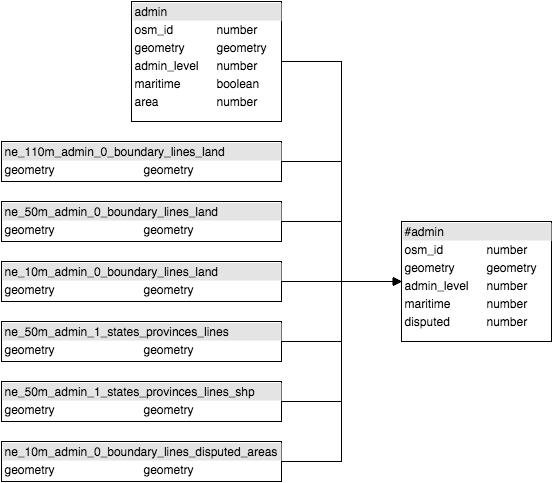
\includegraphics[scale=0.6]{images/admin_layer.png}
  \caption{Layers for administrative areas}
\end{figure}

\newpage
\subsection{Roads, Bridges and Tunnels}
Roads are split up into normal roads, tunnels and bridges after a certain zoom level. \texttt{z\_order} and \texttt{layer} attributes are used to order the geometries on the right z axis.

\begin{figure}[h]
  \centering
  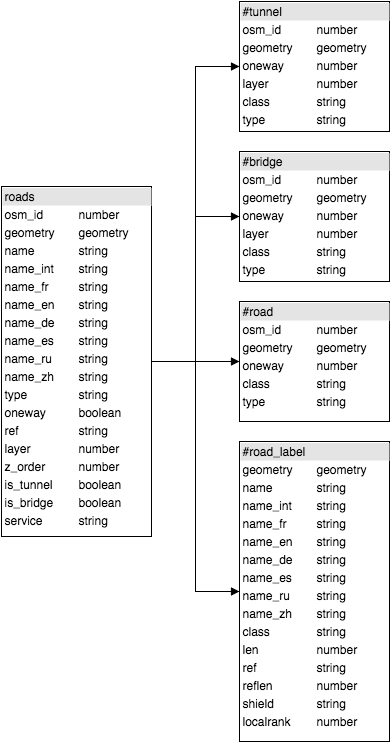
\includegraphics[scale=0.6]{images/road_layer.png}
  \caption{Layers for roads, tunnels and bridges}
\end{figure}

\newpage
\subsection{Points of Interest}
Most POIs are in fact points but buildings tagged with POI attributes
are often polygons, which is why we need to create tables for both points and polygons.
The \texttt{localrank} and \texttt{scalerank} of the \texttt{\#poi\_label} layer are calculated from the \texttt{type} and \texttt{area} attributes.
The \texttt{address} field is pulled together from the various address attributes on the tables (\texttt{street}, \texttt{housenumber}, \texttt{place}, \texttt{city}, \texttt{postcode} and \texttt{country}).

\begin{figure}[h]
  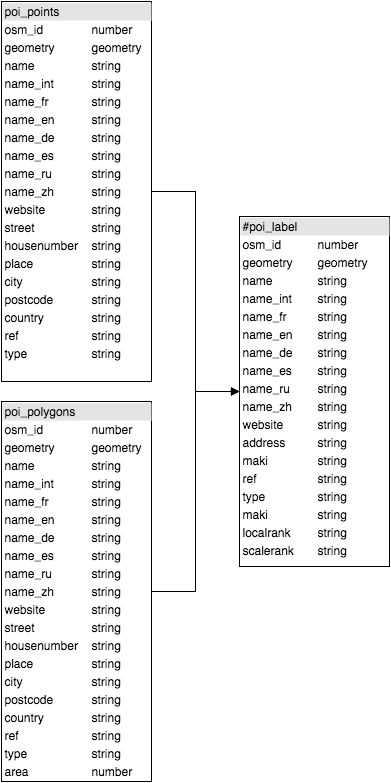
\includegraphics[scale=0.6]{images/poi_layer.png}
  \caption{Point of interest label layer}
\end{figure}


\newpage
\subsection{Water}
Water bodies for lower zoom levels are taken from Natural Earth
data while lakes and rivers are from \osm{}.

\begin{figure}[h]
  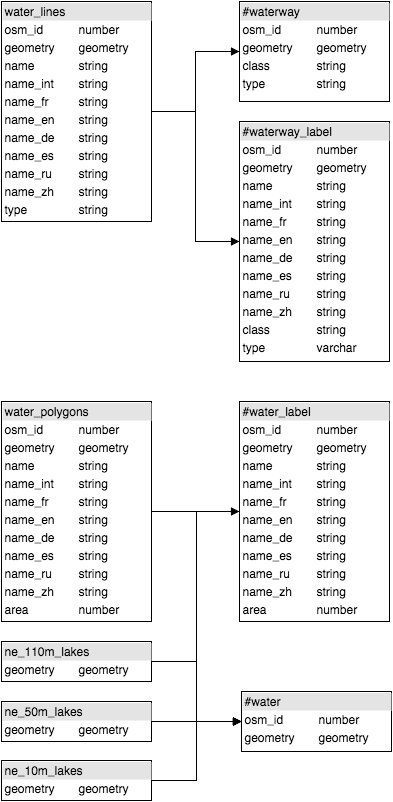
\includegraphics[scale=0.6]{images/water_layer.png}
  \caption{Water bodies and river layers}
\end{figure}



\newpage
\subsection{Places}
The original \osm{} place data is enriched with scalerank data
from natural earth.

\begin{figure}[h]
  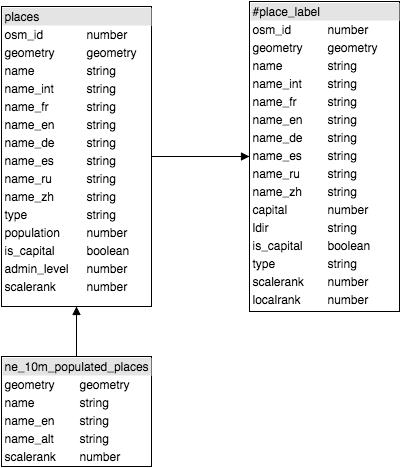
\includegraphics[scale=0.6]{images/place_layer.png}
  \caption{Place label layer}
\end{figure}



%------------------------------------------------------
\newpage
\section{Package Diagrams}

\subsection{Import}

The entire import process is a combination of different smaller imports of different datasources.

\paragraph{import-osm-data}
Import of the OSM planet file with imposm 3 and a custom mapping configuration.

\paragraph{import-sql}
Custom SQL functions that make querying easier and generated SQL code for
classifications.

\paragraph{import-natural-earth}
Import of Natural Earth data.

\paragraph{import-scaleranks}
Custom scalerank updates from Natural Earth data for better scaleranks in places.

\paragraph{import-water}
Water polygons from OpenStreetMapData.

\begin{figure}[h]
  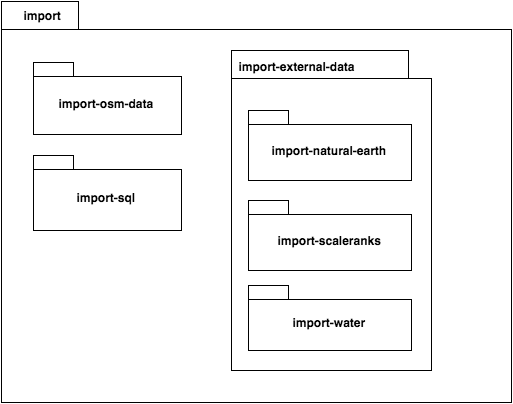
\includegraphics[scale=0.6]{images/import_package.png}
  \caption{Import package}
\end{figure}

\newpage
\subsection{Export}
Export can either be done locally which will process one bounding box or
split up into several machines using remote features.

\paragraph{open-streets.tm2source}
The data style project is the most essential component which pulls together all the
data of different datasources to create vector tile. 

\paragraph{export-local}
A process which is using the open-streets.tm2source project to create vector tiles for a
given bounding box.

\paragraph{export-remote}
A worker implementation which uses a queue to read jobs and work through jobs with
export-local.

\paragraph{enqueue-jobs}
Create jobs for certain areas automatically.

\paragraph{merge}
Merge results of jobs together into a final big file.

\begin{figure}[h]
  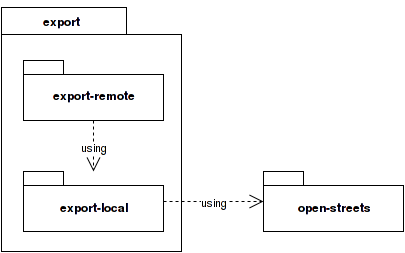
\includegraphics[scale=0.6]{images/export_package.png}
  \caption{Export package}
\end{figure}
\newpage